\documentclass{article} % For LaTeX2e
\usepackage{nips14submit_e,times}
\usepackage{amsmath}
\usepackage{amsthm}
\usepackage{amssymb}
\usepackage{mathtools}
\usepackage{hyperref}
\usepackage{url}
\usepackage{algorithm}
\usepackage[noend]{algpseudocode}
%\documentstyle[nips14submit_09,times,art10]{article} % For LaTeX 2.09

\usepackage{bbm}
\usepackage{graphicx}
\usepackage{caption}
\usepackage{subcaption}
\usepackage{MnSymbol}

\def\eQb#1\eQe{\begin{eqnarray*}#1\end{eqnarray*}}
\def\eQnb#1\eQne{\begin{eqnarray}#1\end{eqnarray}}
\providecommand{\e}[1]{\ensuremath{\times 10^{#1}}}
\providecommand{\pb}[0]{\pagebreak}
\DeclarePairedDelimiter\ceil{\lceil}{\rceil}
\DeclarePairedDelimiter\floor{\lfloor}{\rfloor}

\newcommand{\E}{\mathrm{E}}
\newcommand{\Var}{\mathrm{Var}}
\newcommand{\Cov}{\mathrm{Cov}}
\newcommand\eqD{\stackrel{\mathclap{\normalfont\mbox{d}}}{=}}

\def\Qb#1\Qe{\begin{question}#1\end{question}}
\def\Sb#1\Se{\begin{solution}#1\end{solution}}

\newenvironment{claim}[1]{\par\noindent\underline{Claim:}\space#1}{}
\newtheoremstyle{quest}{\topsep}{\topsep}{}{}{\bfseries}{}{ }{\thmname{#1}\thmnote{ #3}.}
\theoremstyle{quest}
\newtheorem*{definition}{Definition}
\newtheorem*{theorem}{Theorem}
\newtheorem*{lemma}{Lemma}
\newtheorem*{question}{Question}
\newtheorem*{preposition}{Preposition}
\newtheorem*{exercise}{Exercise}
\newtheorem*{challengeproblem}{Challenge Problem}
\newtheorem*{solution}{Solution}
\newtheorem*{remark}{Remark}
\usepackage{verbatimbox}
\usepackage{listings}
\usepackage{mathrsfs}
\title{ProbLimI: \\
Problem Set VI}


\author{
Youngduck Choi \\
CIMS \\
New York University\\
\texttt{yc1104@nyu.edu} \\
}


% The \author macro works with any number of authors. There are two commands
% used to separate the names and addresses of multiple authors: \And and \AND.
%
% Using \And between authors leaves it to \LaTeX{} to determine where to break
% the lines. Using \AND forces a linebreak at that point. So, if \LaTeX{}
% puts 3 of 4 authors names on the first line, and the last on the second
% line, try using \AND instead of \And before the third author name.

\newcommand{\fix}{\marginpar{FIX}}
\newcommand{\new}{\marginpar{NEW}}

\nipsfinalcopy % Uncomment for camera-ready version

\begin{document}


\maketitle

\begin{abstract}
This work contains solutions to the exercises of the problem set V. The
chosen problems are 1,2, and 3.
\end{abstract}

\bigskip

\begin{question}[1]
\hfill
\begin{figure}[h!]
  \centering
    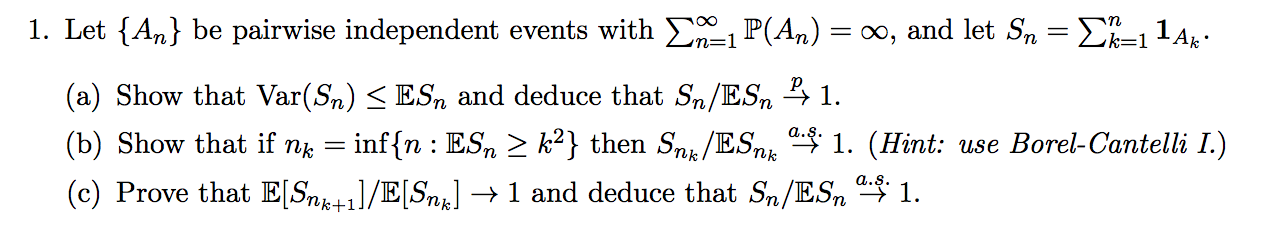
\includegraphics[width=0.7\textwidth]{prob-e6-p1.png}
\end{figure}
\end{question}
\begin{solution} \hfill \\
Observe that 
\eQb
\sum_{k=1}^{n} \mathbb{P}(A_k) &=& \mathbb{E}[S_n]  
\eQe 
for any $n \in \mathbb{N}$. As the LHS tends to $\infty$ as $n \to \infty$, 
we can choose $N$ large enough such that
$\mathbb{E}[S_n] > 0$ for all $n \geq N$. We relabel the indices to start from
$N$ so that the random variables $\{ \dfrac{S_n}{\mathbb{E}[S_n]}\}$ are well-defined
for the problem. 

\bigskip

\textbf{(i)} By independence,
\eQb
\Var(S_n) &=& \sum_{k=1}^{n} \Var(1_{A_k}) = \sum_{k=1}^{n} \mathbb{E}[1_{A_k}^2]
- \mathbb{E}[1_{A_k}]^2 = \sum_{k=1}^{n} \mathbb{P}(1_{A_k}) - 
\mathbb{P}(1_{A_k})^2 \\
&\leq& \sum_{k=1}^{n} \mathbb{P}(1_{A_k}) = \mathbb{E}[S_n]  
\eQe
for each $n \geq 1$. Now, we prove the claimed convergence in probability.
Let $\epsilon > 0$. By Chebyshev's inequality and the above result,
\eQb
\mathbb{P}(|\dfrac{S_n}{\mathbb{E}[S_n]} -1 | > \epsilon) &=&
\mathbb{P}(|S_n - \mathbb{E}[S_n]| > \epsilon \mathbb{E}[S_n]) \\
&\leq& \dfrac{\Var(S_n)}{\epsilon^2  \mathbb{E}[S_n]^2} \leq \dfrac{1}{\epsilon^2
\mathbb{E}[S_n]} 
\eQe
for any $ n \in \mathbb{N}$. Therefore, taking $n \to \infty$, 
\eQb
\lim_{n \to \infty} \mathbb{P}(|\dfrac{S_n}{\E[S_n]} - 1| > \epsilon) &=& 0.
\eQe
Since $\epsilon > 0$ was arbitrary, $\dfrac{S_n}{\E[S_n]} \to 1$ in probability. 

\bigskip

\textbf{(ii)} As $\mathbb{E}[S_n]$ tends to $\infty$ as $n \to \infty$, 
we can find a subsequence with the given property. 
Let $\epsilon > 0$. By the same argument as above, and the property
of the chosen subsequence, 
\eQb
\mathbb{P}(|\dfrac{S_n}{\mathbb{E}[S_n]} - 1| > \epsilon) &\leq& 
\dfrac{1}{\epsilon^2 \mathbb{E}[S_n]} \leq \dfrac{1}{\epsilon^2 k^2}  
\eQe
for all $k \in \mathbb{N}$, which implies
\eQb
\sum_{k=1}^{\infty} \mathbb{P}(|\dfrac{S_{n_k}}{\mathbb{E}[S_{n_k}]} - 1| > 
\epsilon) < \infty.
\eQe
By Borel-Cantelli I, 
\eQb
\mathbb{P}(|\dfrac{S_{n_k}}{\mathbb{E}[S_{n_k}]} - 1| > \epsilon \>\>\>\> i.o) &=& 0
\eQe
for any $\epsilon > 0$. Now, by definition of pointwise convergence,
\eQb
\mathbb{P}(\dfrac{S_{n_k}}{\mathbb{E}[S_{n_k}]} \to 1) &=& 
\mathbb{P}(\bigcap_{\epsilon > 0} \{|\dfrac{S_{n_k}}{\mathbb{E}[S_{n_k}]} - 1|
< \epsilon \>\> \text{a.a} \} ) 
= 1 - \mathbb{P}(\bigcup_{\epsilon > 0} \{ |\dfrac{S_{n_k}}{\mathbb{E}[S_{n_k}]} - 1|
\geq \epsilon \>\> \text{i.o.} \} )   
\eQe
By density of rationals and the above result,
\eQb
\mathbb{P}(\bigcup_{\epsilon > 0} \{ |\dfrac{S_{n_k}}{\mathbb{E}[S_{n_k}]} - 1|
\geq \epsilon \>\> \text{i.o.} \} )  
&=& \mathbb{P}(\bigcup_{\epsilon > 0; \epsilon \in \mathbb{Q}}
\{ |\dfrac{S_{n_k}}{\mathbb{E}[S_{n_k}]} - 1| \geq \epsilon \>\> \text{i.o.}\}) \\ 
&\leq&
\sum_{\epsilon > 0; \epsilon \in \mathbb{Q}}
\mathbb{P}(
|\dfrac{S_{n_k}}{\mathbb{E}[S_{n_k}]} - 1| \geq \epsilon \>\> \text{i.o.}) = 0 
\eQe
and hence
\eQb
\dfrac{S_{n_k}}{\mathbb{E}[S_{n_k}]} &\to& 1 \>\>\> \text{almost surely}.
\eQe

\end{solution}

\newpage

\begin{question}[2]
\hfill
\begin{figure}[h!]
  \centering
    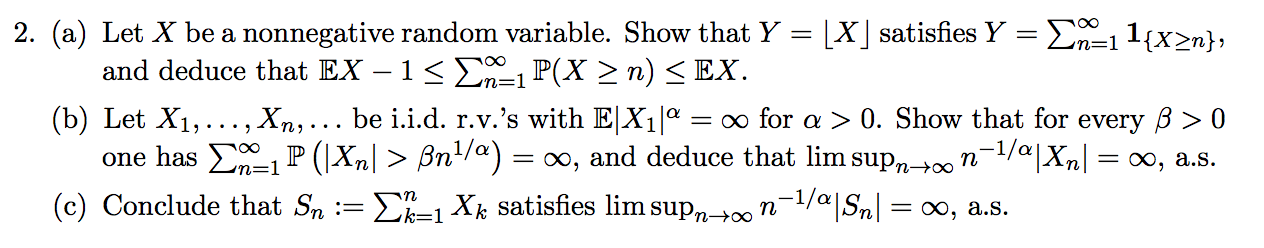
\includegraphics[width=0.7\textwidth]{prob-e6-p2.png}
\end{figure}
\end{question}
\begin{solution} \hfill \\
\textbf{(a)} As $X$ is non-negative real-valued RV and
$1_{\{ X \geq n \} }(w) = 0$ for each $n > \max\{k \in \mathbb{N} 
\> : \> k \leq X(w) \}$. 
\eQb 
\lfloor X(w) \rfloor &=& 
\max\{k \in \mathbb{N} \> : \> k \leq X(w) \} = \sum_{n=1}^{\max\{
k \in \mathbb{N} \> : \> k \leq X(w) \}} 1_{\{X \geq n\}}(w) 
= \sum_{n=1}^{\infty} 1_{\{X \geq n\}}(w) 
\eQe
for any $w \in \Omega$, and hence
\eQb
\lfloor X \rfloor &=& \sum_{n=1}^{\infty}1_{\{ X \geq n\}} = Y.
\eQe 
Observe that $\{\sum_{n=1}^k 1_{\{X \geq n\}}\}_{k}$ is a pointwise
non-decreasing and non-negative sequence of RVs, which converges pointwise
everywhere to $Y = \lfloor X \rfloor$.
Hence, by MCT,
\eQb
\mathbb{E} Y &=& \sum_{n=1}^{\infty} \mathbb{E} 1_{\{X \geq n\}} 
= \sum_{n=1}^{\infty} \mathbb{P}(X \geq n).
\eQe 

Since $X - 1 \leq \lfloor X \rfloor \leq X$, if $X$ is integrable, 
by monotonicity of integration,
\eQb
\mathbb{E}[X] - 1 &\leq& \sum_{n=1}^{\infty} \mathbb{P}(X \geq n) \leq 
\mathbb{E}[X].
\eQe
If $\mathbb{E}[X] = \mathbb{E}[X] - 1 = \infty$, 
then $X-1$ is not integrable, as otherwise it will contradict the non-integrability of
$X$ by linearity. Therefore, $\mathbb{E}[Y] = \mathbb{E}[X-1] = \infty$, so
the inequality holds trivially. 

\bigskip

\textbf{(b)} Let $\beta > 0$. Observe that
\eQb
\sum_{n=0}^{\infty} 1_{\{\beta^{-\alpha} |X_1|^{\alpha} > n\}} &=& 
\lceil \beta^{-\alpha}|X_1|^{\alpha} \rceil.
\eQe 
Similar to (a), by MCT,
\eQb
\sum_{n=0}^{\infty} \mathbb{P}(\beta^{-\alpha} |X_1|^{\alpha} > n ) 
&=& \mathbb{E}\lceil \beta^{-\alpha}|X_1|^{\alpha} \rceil . 
\eQe
We now have the following pointwise estimate:
\eQb
\beta^{-\alpha} |X_1|^{\alpha} &\leq& \lceil \beta^{-\alpha} |X_1|^{\alpha} \rceil. 
\eQe
As $\mathbb{E}|X_1|^{\alpha} = \infty$, we see $\mathbb{E}[\beta^{-\alpha}|X_1|^{\alpha}]
= \infty$ and combined with the above estimate 
\eQb
\sum_{n=0}^{\infty} \mathbb{P}(|X_n| > \beta n^{\frac{1}{\alpha}}) = 
\sum_{n=0}^{\infty} \mathbb{P}(\beta^{-\alpha} |X_1|^{\alpha} > n ) &=&
\infty
\eQe
which implies
\eQb
\sum_{n=1}^{\infty} \mathbb{P}(|X_n| > \beta n^{\frac{1}{\alpha}}) &=& \infty. 
\eQe
Since $\beta > 0$ was arbitrary, we have the result for all $\beta > 0$.

\smallskip

Set
\eQb
A_k &=& \{ n^{-\frac{1}{\alpha}} |X_n| > k \>\>\> \text{ i.o.} \} 
\eQe
for each $k \in \mathbb{N}$. By Borel-Cantelli II, combined with the above result,
\eQb
\mathbb{P}(A_k) = 1
\eQe
for each $k \in \mathbb{N}$. Since $\{ A_k \}$ is descending, by continuity of 
probability,
\eQb
\mathbb{P}(\bigcap_{k=1}^{\infty} A_k) &=& 1.
\eQe
Suppose $w \in \bigcap_{k=1}^{\infty} A_k$. By induction, we construct
a subsequence, which diverges to $\infty$. Choose $n_1$ such that 
\eQb
(n_{1})^{-\frac{1}{\alpha}}|X_{n_1}(w)| > 1.
\eQe
Given $\{n_i\}_{i=1}^{l}$, choose $n_{l+1}$ larger than all previous indices such that 
\eQb
(n_{l+1})^{-\frac{1}{\alpha}}|X_{n_{l+1}}(w)| > l + 1.
\eQe
By induction, we have constructed a subsequence $\{n_l\}$ such that
\eQb
(n_{l})^{-\frac{1}{\alpha}}|X_{n_{l}}(w)| > l
\eQe
for each $l \in \mathbb{N}$, and hence
\eQb
\bigcap_{k=1}^{\infty} A_k &\subset& 
\{ \limsup_{n \to \infty} n^{-\frac{1}{\alpha}} |X_n|  = \infty \}.
\eQe
Therefore, 
\eQb
\limsup_{n \to \infty} n^{-\frac{1}{\alpha}} |X_n| = \infty \>\>\> \text{a.s.}
\eQe

\bigskip

\textbf{(c)}

\end{solution}

\newpage

\begin{question}[3]
\hfill
\begin{figure}[h!]
  \centering
    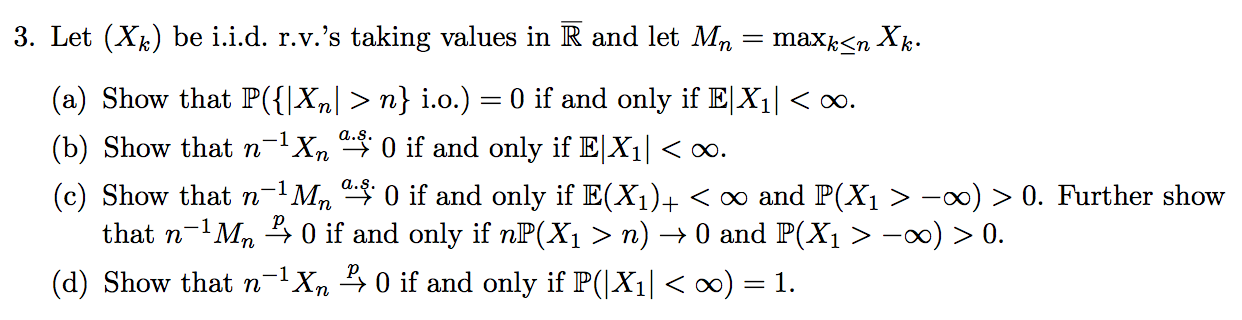
\includegraphics[width=0.7\textwidth]{prob-e6-p3.png}
\end{figure}
\end{question}
\begin{solution} \hfill \\
\end{solution}

\newpage

\begin{question}[4]
\hfill
\begin{figure}[h!]
  \centering
    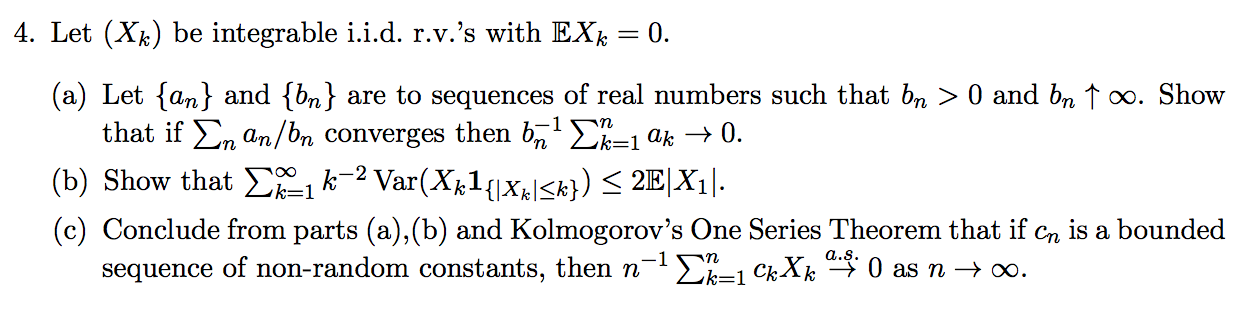
\includegraphics[width=0.7\textwidth]{prob-e6-p4.png}
\end{figure}
\end{question}
\begin{solution} \hfill \\
\textbf{(a)}
Let $b_0, s_0  = 0$ and
$s_n = \sum_{k=1}^{n} \dfrac{a_n}{b_n}$, so $a_n = b_n(s_n - s_{n-1})$ for each $n 
\in \mathbb{N}$.
Observe that
\eQb
\dfrac{1}{b_n}\sum_{k=1}^{n} a_n &=& \dfrac{1}{b_n} \sum_{k=1}^{n}
b_k(s_k - s_{k-1}) = s_n - \sum_{k=1}^{n} (\dfrac{b_k - b_{k-1}}{b_n}) s_{k-1}  
\eQe 
for each $n \in \mathbb{N}$. Let $s_{\infty}$ be the limit of $\{s_n\}$. It suffices
to show that the right most term on the above formula converges to $s_{\infty}$.
Let $\epsilon > 0$. By triangle inequality,
\eQb
|\sum_{k=1}^{n} (\dfrac{b_k - b_{k-1}}{b_n}) s_{k-1} - s_{\infty}| 
&\leq& \sum_{k=1}^{n} (\dfrac{b_k - b_{k-1}}{b_n}) |s_{k-1} - s_{\infty}| \\
&=& \sum_{k=1}^{m} (\dfrac{b_k - b_{k-1}}{b_n})|s_{k-1} - s_{\infty}| 
+ \sum_{k=m+1}^{n} (\dfrac{b_k - b_{k-1}}{b_n})|s_{k-1} - s_{\infty}|  
\eQe  
for each $1 \leq m < n$. Choose $m_0$ such that $|s_{n} - s_{\infty}| < \epsilon$ for
each $n \geq m_0$. Then 
\eQb
|\sum_{k=1}^{n} (\dfrac{b_k - b_{k-1}}{b_n}) s_{k-1} - s_{\infty}| 
&\leq& \dfrac{1}{b_n} \sum_{k=1}^{m_0} 
(b_k - b_{k-1})|s_{k-1} - s_{\infty}| 
+ \dfrac{b_n - b_{m_0}}{b_n} \epsilon  
\eQe 
for each $n \geq m_0$. Letting $n \to \infty$,
\eQb
|\sum_{k=1}^{n} (\dfrac{b_k - b_{k-1}}{b_n}) s_{k-1} - s_{\infty}| < \epsilon 
\eQe
as required.

\bigskip

\textbf{(b)} 

\bigskip

\textbf{(c)} 

\end{solution}
\end{document}
